\documentclass[a4paper,4pt]{article}
\usepackage[utf8]{inputenc}
\usepackage{graphicx}
\usepackage{sidecap}
\usepackage{amsmath}
\usepackage[T1]{fontenc}
\usepackage[italian]{babel}
\usepackage{geometry}
\usepackage{booktabs}
\usepackage{color}
\usepackage{xcolor}
\usepackage{gensymb}
\usepackage{colortbl}
\usepackage{wrapfig}
\usepackage{floatflt,epsfig}
\usepackage[]{subfig}
\usepackage[]{caption}
\usepackage{listings}
\usepackage[hidelinks]{hyperref}
\usepackage[pdf]{graphviz} 
\graphicspath{{7-02-2019/},{4-02-2019/},{11-02-2019/}}
\setlength{\parskip}{10pt plus 1pt minus 1pt}
\definecolor{xanadu}{rgb}{0.45, 0.53, 0.47}
\usepackage{amssymb}
\lstset{
    language=JAVA, %% Troque para PHP, C, Java, etc... bash é o padrão
    basicstyle=\ttfamily\small,
    numberstyle=\footnotesize,
    numbers=left,
    backgroundcolor=\color{gray!10},
    frame=single,
    tabsize=2,
    rulecolor=\color{black!30},
    title=\lstname,
    escapeinside={\%*}{*)},
    breaklines=true,
    breakatwhitespace=true,
    framextopmargin=2pt,
    framexbottommargin=2pt,
    inputencoding=utf8,
    extendedchars=true,
    showstringspaces = false,
    literate={á}{{\'a}}1 {ã}{{\~a}}1 {é}{{\'e}}1 {è}{{\'e}}1 {ò}{{\'o}}1  {ù}{{\'u}}1 {à}{{\'a}}1 ,   
    commentstyle=\color{xanadu},
}

\begin{document}



\tableofcontents


\newpage
\section{4-02-2019: INTRO}
\textbf{DICHIARAZIONE $\neq$ ASSEGNAMENTO} \newline
L'assegnamento fa riferimento alla modifica di una variabile.
\begin{lstlisting}[basicstyle=\small,]

int n		   /* Dichiarazione */
int m = n = 1; /* Inizializzazione */
n = 2 		   /* Assegnamento */

\end{lstlisting}

\noindent \textbf{PROGRAMMAZIONE IMPEATTIVA VS FUNZIONALE} \newline
JAVA è un linguaggio \textit{imperattivo} ad oggetti. Questo significa che si programma variando lo stato interno delle varie istanze. In contrapposizione troviamo la programmazione funzionale che si basa sul richiamare e scrivere funzioni che non variano gli stati interni delle istanze. Nella programmazione funzionale sono usati spesso metodi che ritornano copie modificate di un determinato oggetto, senza modificare l'oggetto attuale.

\noindent \textbf{JAVA VIRTUAL MACHINE} \newline
\noindent Java è stato realizzato con un compilatore integrato, che non compila in assembly, questo compilatore invece produce un file sorgente che non è eseguibile direttamente dalla macchina, bensi è eseguibile da una virtual machine, la JVM(\textit{java virtual machine}). In questo modo viene garantita la portabilità del codice in vari computer con CPU diversa (come il Phyton e .NET). \newline
Questa separazione non conta niente per il linguaggio, si riflette solamente sul modello architetturale.

\noindent U.M.L. = unified model language $\Rightarrow$ rappresentazioni di gerarchie di classi. \newline
\digraph{ao}{rankdir=LR;

   a [label="Animali" shape = "record"]; 
   c [label="Cani" shape = "record"]; 
   g [label="Gatti" shape = "record"]; 
   d [label="Dalmata" shape = "record"]; 
   c->a; g->a; d->c;} \newline
\textbullet\ Tutte le sottoclassi sono dei sottoinsiemi. \newline
\textbullet\ Tutte le superclassi sono dei sovrainsiemi. 

\noindent I linguaggi ad oggetti ci permettono di costruire \textit{tipi} e di definire \textit{valori}. 
\begin{lstlisting}[basicstyle=\small,]
	Animale a = new Animale();
	/* in Java gli oggetti sono valori
	 * dove: Animale -> tipo -> CLASSE
	 * a = nome variabile
	 * new Animale() ha un valore -> OGGETTO */
\end{lstlisting}

\noindent \textbf{COMPILING TIME E RUNTIME} \newline
La gestione di sintassi e di errori viene fatta in due fasi.
Dal compilatore(compiling time): \newline
\textbullet\ Viene eseuito un controllo sintattico \newline
\textbullet\ Viene eseguito controllo dei tipi, cioè che gli insiemi siano corretti\newline
In fase di esecuzione(RunTime):\newline
\textbullet\ Abbiamo a che fare con valori e non con tipi, vengono controllati i "cast"

\noindent I tipi di fatto sono una astrazione del linguaggio. \newline
Il senso di un compilatore è quello di evitare di scrivere castonerie che a livello di esecuzione non avrebbero senso.

\noindent \textbf{SOUNDNESS} \newline
Un linguaggio si dice \textit{sound} quando il compilatore ti da la certezza che in fase di esecuzione il programma sia eseguito correttamente senza possibilità di errori.

\noindent \textbf{PARAMETRO IMPLICITO} \newline
 Ogni metodo dichiarato ha sempre un parametro implicito (il parametro \textit{this}). Esso è sotto inteso e viene passato automaticamente, più eventuali parametri che vengono passati all'interno del metodo.
\begin{lstlisting}[basicstyle=\small,]
	public class Animal {
		private int peso;
		...
		public void mangia(Animali a){
			this.peso = this.peso + a.peso;
		}
	}
	
	Cane fido = new Cane();
	a.mangia(fido); 			/* SUBSUMPTION (assunzione)	*/
\end{lstlisting}

\noindent \textbf{POLIMORFISMO} \newline
L'eredità è un meccanismo che garantisce il funzionamento del \textit{polimorfismo}.\newline
\textbullet\ Polimorfismo per \textit{SUBTYPING} o anche polimorfismo per inclusione: si riferisce al fatto che una espressione il cui tipo sia descritto da una classe A può assumere valori di un qualunque tipo descritto da una classe B sottoclasse di A (Vedi codice appena sopra)\newline 
\textbullet\ Polimorfismo dei \textit{GENERICS}: si riferisce al fatto che il codice del programma può ricevere un tipo come parametro invece che conoscerlo a priori (polimorfismo parametrico). In questo modo non si perde il tipo originario passato dall'oggetto al metodo \newline
\begin{lstlisting}[basicstyle=\small,]
	/* POLIMORFISMO SUBTYPING
	 * basato sui sottotipi ereditarietà */
	Object ident (Object x){
		return x;
	}

	/* POLIMORFISMO GENERICS (parametrico)
	 * non perdo informazioni sui tipi */
	<T> T ident (T x){
		return x;
	}
	/* questa funzione mi permette di riusare il 
	 * metodo, in questo modo evito di fare CAST,
	 * e di sbagliare a farli */
\end{lstlisting}

\newpage




\newpage
\section{7-02-2019: DINAMIC DISPATCHING}
Nei linguaggi ad oggetti, lo strumento più potente è la classe. Quando definisco le entità che poi vado a tramutare in classi sto definendo DATI. \newline
Le classi possono contenere dei metodi (funzioni che operano sugli oggetti della classe). \newline
Definire sottoclassi significa definire \textit{sottoinsiemi} nell'ambito dell'ereditarietà. Le nuove operazioni delle sottoclassi vanno inserite sapendo che le sottoclassi ereditano il set di funzioni delle superclassi. 
\textit{IL POLIMORFISMO} è uno strumento molto utile perchè ci permette di scrivere codice, funzioni che posso adoperare anche con tipi diversi! \newline
@ serve per creare delle annotazioni nel codice, serve per il compilatore (es: @ override).

\noindent \textbf{OVERRIDING} \newline
L'\textit{Overriding} è il punto cruciale di tutta la programmazione ad oggetti. Fare overriding significa sovrascrivere un metodo ereditato dalla super classe per poterne specializzare il suo comportamento. Se non potessi farlo significa che nelle sottoclassi non posso andare a specializzare un metodo. Specializzare un metodo significa cambiare l'implementazione della super classe senza cambiarne la firma. 


\noindent \textbf{DINAMIC DISPATCHING} \newline
Il \textit{Dinamic dispatching} serve in fase di runtime a scegliere la versione giusta del metodo da richiamare. Infatti se ho degli over ride nelle mie classi, sarà solo in fase di run time che Java deciderà quale metodo richiamare. Se nella mia classe non esiste il metodo richiamato, il dinamic dispatching va a prendere l'implementazione del metodo dalla superclasse. Nella memoria che contiene le informazioni degli oggetti ci sono tutti i puntatori ai metodi di una classe, in run time viene eseguito il codice del puntatore corretto. (\textit{vedere: virtual table}).
Un \textit{OGGETTO} infatti è costituito da un insieme dei suoi campi e da puntatori ai metodi della classe ed è grazie a questo che il dispatching funziona: il compilatore controlla i tipi e garantisce che nel compiling time tutto questo funzioni. 

\noindent Ogni espressione ha un tipo!

\noindent \textbf{CLASSI E METODI STATICI} \newline
\textbullet\ I metodi statici sono quei metodi di una classe che appartengono alla classe, non alle istanze di una classe. Si possono richiamare senza creare un oggetto. I metodi statici possono quindi accedere solo a dati statici e non alle variabili di istanza della classe, possono solo richiamare altri metodi statici della classe, e sopratutto non possono usare il parametro implicito \textit{this}. \newline
\textbullet\ Le classi statiche in java possono solamente esistere se sono \textit{innestate (nested)}. Esse possono accedere solamente dati statici della classe che le contiene. Una classe statica interna non vede il riferimento this dell'altra classe, essa può accedere solamente ai campi statici della classe che la contiene.\newline
Le classi statiche non sono però come i membri statici, è possibile infatti instanziarne più istanze, tutte quante indipendenti e non relazionate tra di loro. 

\noindent \textbf{COLLECTION} \newline
Le \textit{Collection o contenitori} sono delle interfacce della libreria di JAVA e non si possono costruire.\newline
Le \textit{Collection} da sole non sono dei tipi, le \textit{Collection} di un "qualcosa" sono dei tipi.I tipi parametrici vogliono infatti un \textit{argomento} \newline
\begin{center}
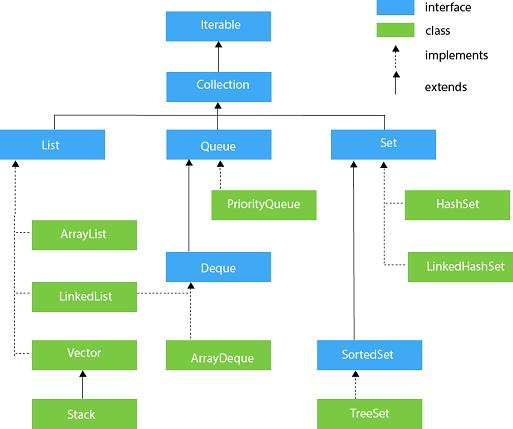
\includegraphics[width=%
0.6\textwidth]{java-collection-hierarchy}
\end{center} 

\noindent \textbf{PACCHETTI JAVA}\newline
JAVA SE $\Rightarrow$ Standard Edition \newline
JAVA EE $\Rightarrow$ Enterprise Edition \newline
JAVA ME $\Rightarrow$ Mobile Edition \newline
JAVA JDK $\Rightarrow$ linguaggio + tutte le librerie standard (java developement kit) \newline
JAVA JRE $\Rightarrow$ Solo a runtime, versione ridotta che serve solo a chi usa i programmi ma non al programmatore (java runtime enviroment) \newline
File jar  $\Rightarrow$ Archivio di tutti i pacchetti del programma \newline
JAVA JVM $\Rightarrow$ (Java virtual machine) serve per eseguire i file .jar \newline
La documentazione di java si trova on-line ed è diffusa in pacchetti che servono ad organizzare logicamente le classi, che sono organizzate in ordine alfabetico. \newline





\newpage













\newpage
\section{11-02-2019: ITERATORI E GENERICS}
\textbullet\  \textit{ITERATORE}: E' un pattern, uno stile di programmazione. Il pattern degli iteratori esiste in tutti i linguaggi ad oggetti. Con iteratore intendiamo lo scorrimento di una collezione di elementi. L'iteratore serve quindi a scorrere una collection.\newline
\textbullet\ \textit{ITERABLE}: E' una super interfaccia, e l'interfaccia \textit{COLLECTION} implementa questa super interfaccia. Iterable è super tipo di tutte le interfacce.

\noindent Se una interfaccia rappresenta una super interfaccia significa che non ha un genitore, anche se in realtà estende \textit{Object}


\noindent \textbf{MAPPA}\newline
Una mappa è una struttura dati che mappa chiavi e valori, ha quindi due parametri: il tipo della chiave e il tipo del valore. Una mappa è una \textit{collection} solo se vista come una collection di coppie. Infatti una \textit{collection} è figlia di \textit{iterable} (la posizione più alta nella gerarchia), ma una \textit{mappa} NON è figlia di \textit{iterable}
\begin{center}
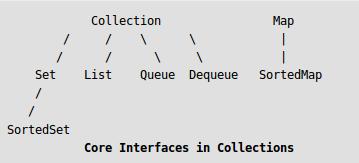
\includegraphics[width=%
0.6\textwidth]{MapInterface}
\end{center} 
Ci riferiamo ad un oggetto usando la parola \textit{sottotipo} quando esso è:\newline
\textbullet\ O una sottoclasse (extends) \newline
\textbullet\ O una sotto interfaccia (implements) \newline
Ad esempio ArrayList ha come superclasse abstract arrayList. ArrayList implementa collection. Quindi ne è sottotipo ma non sottoclasse.

\noindent \textbf{GENERICS}\newline
<? extends classe> rappresenta un tipo. \newline
<? extends E> \newline
La \textit{SUBSUMPTION} non funziona tra GENERICS. Per il parametro stesso c'è subsumption, ma non per le collection. Il tipo con il ? accetta sottotipi di parametri.\newline
\textbullet\ Il TIPO ESTERNO gode sempre della la subsumption, 
\textbullet\ Il TIPO INTERNO non gode mai della subsumption, la subsumption si può fare solo usndo i generics( quindi con <? extends E>)  \newline
[Invarianza del subtyping]: Se ciò non fosse le subsumption funzionerebbero anche nel tipo interno e questo rischierebbe la totale spaccatura \newline
Se cosi non fosse in java non verrebbero mai rispettate le regole delle classi. \newline
Java di unico ha che esiste il wildchart (?), che è un modo controllato per risolvere il problema della subsumption dei tipi interni. \newline
Prima dei generics (2003/2004) in java si programmava tutto a typecast. Per motivi di retrocompatibilità è possibile programmare in tutti e due i modi. E' comunque consigliato usare la porgrammazione con i \textit{generics}. \newline
Metodi che ritornano un booleano iniziano con sempre come se fossero domande; es: hasNext, isEmpty etc.. \newline
Un iteratore non può essere costruito con un new perchè è un'interfaccia. 
\newpage


 
\newpage
\section{15-02-2019}
\textbf{INTERFACCE}\newline
\begin{lstlisting}[basicstyle=\small,]
	public interface Iterator<T>{}
\end{lstlisting}
L'interfaccia è un contratto, nel senso che mette a disposizione una serie di metodi che ogni classe che estende quell'interfaccia deve obbligatoriamente implementare, pena un errore durante la fase di compilazione.In java quindi si può scrivere del codice ancora prima di sapere come si potrebbe implementare.

\noindent Facciamo un esempio: il "contratto" di iteratore è il seguente: \newline
\textbullet\ boolean hasNext(); \newline
\textbullet\ T next(); \newline
\textbullet\ void remove()\newline
Data una certa classe che può non essere sotto al nostro controllo non abbiamo bisogna sapere necessariamente come sono stati implementati i suoi metodi, ma ci ti basta sapere che esistono per poter dire se sia o meno un iteratore. \newline
Esempio di definizione di un metodo con iteratore come input: 
\begin{lstlisting}[basicstyle=\small,]
	public statics void scorri(Iteratore <Integer> it){
		while(it.hasnext()){
			integer n = it.next();
		}
	}
\end{lstlisting}
Esempio di utilizzo 
\begin{lstlisting}[basicstyle=\small,]
	scorri(new Iterator<>(){
		...
		...
		...
	});
\end{lstlisting}
Quest'ultima è un'espressione, o come meglio dire, un'oggetto fatto al volo. Questa sintassi è stata creata appositamente per le interfacce (dato che non si possono istanziare direttamente), senza dover andare a definire una classe con la classica implementazione dell'interfaccia. 

\noindent \textit{ANONYMOUS CLASS} meccanismo comodo per design pattern come le call-back. 

\noindent Questa implementazione garantisce che la funzione sia \textit{SOUND}, e non crasherà mai a \textit{RunTime}

\noindent \textbf{IMPLEMENTARE INTERFACCE}\newline
1) Con implements: \newline
\textbullet\ controlla i metodi che hai implementato all'interno della classe \newline
\textbullet\ assicura che siano implementati tutti 

\noindent Tipi delle interfacce \newline
Iterator $\Rightarrow$ non è un tipo \newline
Iterator<T> $\Rightarrow$ è un tipo 

\noindent \textbf{NOTAZIONE BNS} \newline
BNS è il nome della notazione e serve per poter dare delle regole grammaticali. E' una notazione che definisce la sintassi delle espressioni\newline
Iterator da solo, sintatticamente, sarebbe un tipo. Ma il compilatore verifica che non è un tipo e da errore.








\newpage 



\newpage
\section{18-02-2019: CLASSI ASTRATTE}
\textbf{CLASSE ASTRATTA} \newline
Una classe si dice astratta quando ha almeno un metodo astratto, essa serve per impedire la sua costruzione (non posso quindi istanziarla). Delle classi vengono definite astratte se anche un solo metodo è astratto. Una delle maggiori differenze tra classi astratte ed interfacce è che una classe può implementare molte interfacce ma può estendere una sola classe astratta. Una interfaccia è zucchero sintattico di una classe astratta con soli metodi astratti. Zucchero sintattico (Syntactic sugar) è un termine coniato dall'informatico inglese Peter J. Landin per definire costrutti sintattici di un linguaggio di programmazione che non hanno effetto sulla funzionalità del linguaggio, ma ne rendono più facile ("dolce") l'uso per gli esseri umani. La differenza tra classe ed interfaccia in realtà non esiste.

\noindent Un array è una struttura dati lineare, omogenea e contigua in memoria.

\noindent Per leggere una \textit{collection} si usano gli iteratori che servono per farne il get in sequenza.

\noindent \textbf{VTABLE E DIMENSIONE DI UNA CLASSE} \newline
Una virtual Table, o dispatching table, è un meccanismo utilizzato per supportare il dynamic dispatching (o anche chiamato run-time method binding).Quando una classe definisce dei metodi virtuali, il compilatore nasconde all'interno dei membri della classe una variabile che punta ad un array di puntatori a funzioni. Questi puntatori sono poi usati a runtime per invocare l'implementazione della funzione appropiata, questo perchè in compile-time non è detto che si sappia se la funzione richiamata sia quella del tipo definito o sia derivata da un'altra classe.

\begin{lstlisting}[basicstyle=\small,]
public static class Animale(){
	private int peso;
}

public static class Cane extends Animale{
	private String nome;
	public void abbaia(){};
}

public static class PastoreTedesco extends Cane{

}
\end{lstlisting}
Se costruisco un oggetto di tipo PastoreTedesco, esso sarà grande quanto un tipo int (32 bit) ed una stringa (un puntatore).
Il tutto grazie alla virtual table che tiene in memoria i puntatori dei vari campi di uno oggetto.









\newpage
\section{21-02-2019}
\par

\textit{REFLECTION} è una tecnica per conoscere i tipi e il contenuto delle classi  a runtime. \newline
Se voglio conoscere il tipo dell'enclosing class (classe che contiene) posso fare : nome.classe.this.nome \newline

\textit{BINDING} avviene anche con i tipi \newline
I parametri di una funzione sono binding nello scope della funzione.\newline
I type argument fanno binding con i type parameter, esattamente come avviene per le funzioni tra argomenti e parametri. \newline

Quando si programma con i generics si PROPAGANO. \newline

TYPE ERASURE: cancellazione dei tipi: java lo fa quando compila butta via i generics generando classi non anonime e li sostituisce con Object: il motivo è per mantenere la compatiblità con il vecchio codice che non aveva generics. Quindi i generics sono verificati dal compilatore e poi cancellati per eseguire.

















\newpage
\section{25-02-2019}
\par

Se un oggetto ha dei campi esso pesa tanto quanto la dimensione dei campi. \newline
Nei pc a 64 bit i puntatori pesano 8 byte \newline

L'ereditarietà serve anche a modificare i metodi della classe che viene ereditata. E' l'unico modo che abbiamo per modificare delle cose anche se non sappiamo cosa e chi le ha costruite. Sopratutto se non le possediamo. Un esempio è la classe ArrayList, che deve essere ereditata per implementare un motodo che ci permetta di scorrerla all'indietro. \newline


I metodi statici non si possono override perchè non sono presenti nelle virtual table (sono funzioni sciolte). \newline

Regola ereditarietà costruttore: se non definisco nessun costruttore nella sottoclasse è come se chiamassi il costruttore della superclasse SENZA parametro. 









\newpage
\section{28-02-2019: COVARIANZA e CONTROVARIANZA}
\textbf{COVARIANZA e CONTROVARIANZA DEI TIPI }\newline
Scrivendo  $C \leq A$ intendiamo che C è sottotipo di A. Definito l'operatore minore uguale passiamo alle definizioni vere e propie.

\noindent \textbf{VARIANZA} \newline
$C_{1} <\tau_{1}> \leq C_{2}<\tau_{2}> \Leftrightarrow C_{1} \leq C_{2} \bigwedge \tau_{1}\equiv \tau_{2} $
\newline
Questa regola del type system di \textit{java} ci dice che il linguaggio non è COVARIANTE, in quanto i generics non cambiano. 

\noindent \textbullet\ Esempio: ArrayList<cane> $\leq$ List<cane> (sottotipo) \newline
\textbullet\ Esempio: ArrayList<cane> $\nleq$ List<Animali> \newline
L'ultima formula non è covariante, se fosse possibile si avrebbe una doppia subsunzione sul guscio interno e sul tipo esterno \newline

\noindent \textbf{CONTROVARIANZA} \newline
Quando eredito un metodo di una classe posso sovrascriverlo usando l'overriding. Quando lo faccio un linguaggio di programmazione si dice controvariante se mi è possibile far scendere (specializzare) il tipo di ritorno, e al contempo mi è possibile far salire (rendere più generico) l'argomento di ingresso. Vediamo un esempio (\textit{NON VALIDO IN JAVA}):
\begin{lstlisting}
/* Data questa gerarchia di classi: */
  public class Cane extends Animale{
	/* nella classe Cane faccio l'override
 	 * del metodo ereditato dalla classe
 	 * Animale */  
	public Cane m(Cane c){
		return c;
	}
  }
  
 public class PastoreTedesco Extends Cane{
 	@Override
	public PastoreTedesco m(Animale c){
		return new PastoreTedesco;
	}
	/* rispetto al metodo originale
	 * il tipo di ritorno del metodo 
	 *		(PastoreTedesco) scende (sottoclassi)
 	 * il tipo del parametro di ingresso 
 	 * 		(Animale) sale (superclasse) */	
 }
\end{lstlisting}

\noindent Detto questo è bene specificare che Java supporta i solo i tipi di ritorno controvarianti, è possibile controvariare SOLO il tipo di ritorno del metodo, ed è possibile farlo solamente scendendo (sottotipo). Ed è possibile Fare questo nella fase di overriding, non in quella di overloading. In caso di overloading il tipo di ritorno deve essere lo stesso.

\noindent Il seguente è l'esempio corretto in java:
\begin{lstlisting}
public Cane m (Cane c){return c;}

@Override
public PastoreTedesco m(Cane c){return new PastoreTedesco();}
\end{lstlisting}

\noindent \textbf{SOUNDNESS IN JAVA} \newline
\textbullet\ SOUND : un programma che compila può essere eseguito senza errori \newline
\textbullet\ SOUND JAVA: un programma compila e termina, a meno di una eccezione. \newline
Un esempio di SOUND JAVA è il seguente:in java è possibile avvenga un segmentation fault non per un problema di casting, ma solamente se accediamo ad un indice di un array che non abbiamo allocato, quindi il programma termina a meno di una eccezione. Ci sono invece linguaggi dove non esistono gli array, quindi non accadrà mai segmentation fault e il codice terminerà sempre alla fine senza eccezioni, ovviamente senza fare i controlli di semantica. 

\noindent \textbf{WILDCARDS} \newline
\noindent Recentemente è stato inserito un pattern che permette anche in Java la covarianza: sono i generics con i wildcards. 
\begin{lstlisting}
Arraylist<? extends Animale> m = new List<Cane>();
\end{lstlisting}
\noindent Da questo si capisce che la covarianza può essere usata, ma solamente se esplicitata con il wildcard. \newline
Sono molto usati perchè i wildcard non sono tipi del primo ordine, infatti il \textit{tipo} "? extends classe" non esiste!!!Non posso definire una variabile come segue: 
\begin{lstlisting}
? extends Animale m = new Cane();
/* questa sintassi si può usare solo come type argument */
\end{lstlisting}
Significato: permettono la covarianza, sono tipi temporanei che non possono essere scritti nel codice, però possono essere subsunti con il get(). \newline
Un altro DESIGN PATTERN: callback

















\newpage
\section{4-03-2019: CLASSI ANONIME, LAMBDA E FUNZIONI ORDINE SUPERIORE}
\textbf{DESIGN PATTERN} \newline
\textbullet\ Iteratore \newline
\textbullet\ Compact o Callback o Unary function 

\noindent \textbf{CLASSI ANONIME} \newline
Le classi \textit{lambda} servono per fare funzioni al "volo",senza quindi avere il bisogno di implementare delle interfacce in classi separate. Vediamone un esempio:

\begin{lstlisting}[basicstyle=\small,]
interface HelloWorld {
	public void greet();
    public void greetSomeone(String someone);
}

public static void main (String args[]) {
    HelloWorld frenchGreeting = new HelloWorld() {
        String name = "tout le monde";
        public void greet() {
            greetSomeone("tout le monde");
        }
        public void greetSomeone(String someone) {
            name = someone;
            System.out.println("Salut " + name);
        }
    };
}

\end{lstlisting}

\noindent \textbf{LAMBDA ASTRAZIONI} \newline
Le espressioni \textit{lambda} servono per fare funzioni al "volo",senza quindi avere il bisogno di implementare delle interfacce in classi separate, classi anonime e classi innestate. Si ricorda che le espressioni lambda possono essere usate solo per implementare interfacce funzionali (cioè interfacce che possiedono un solo metodo astratto). Vediamone un esempio:

\begin{lstlisting}[basicstyle=\small,]
interface MyString {
	String myStringFunction(String str);
}

public static void main (String args[]) {
	MyString reverseStr = (str) -> {
		String result = "";		
		return result;
	};
	reverseStr.myStringFunction("temp");
}
\end{lstlisting}

\noindent \textbf{FUNZIONI DI ORDINE SUPERIORE} \newline
Sono delle funzioni che prendono delle funzioni come parametri di ingresso 
\begin{lstlisting}[basicstyle=\small,]
/* questa interfaccia è equivalente all'interfaccia java.util.Functional
 * essa infatti espone una serie di funzioni, senza implementazione, tra 
 * cui anche le call-back */
public interface Func<A, B>{
	B execute(A a); 
	
	/* questa è l'unica funzione esposta dall'interfaccia
	 * un altro nome ragionevole per il metodo execute() è apply() 
	 * oppure call() il nome deve ricordare il fatto di richiamare 
	 * la funzione  */
}

/* questa funzione va ad utilizzare la funzione Func definita sopra */
public static <A,B> List<B> map(List<A> I, Func<A,B> f){
	List<B> r = new ArrayList<>();
	for(A x: l)
		r.add(f.execute(x));
	return r;

}
\end{lstlisting}
A e B sono \textit{generics} locali al metodo(e solo al metodo) \newline
I generics sulle classi servono per parametrizzare, non per fare polimorfismo \newline
\begin{lstlisting}[basicstyle=\small,]
public static <A,B> List<B> map(List<A> I, Func<A,B> f){
/* dove in "public static <A,B>" dichiaro i parametri che useremo
 * mentre in "List<a> .. Func <A,B>" "uso" i parametri */
\end{lstlisting}

\noindent Funzione FILTER: 
\begin{lstlisting}[basicstyle=\small,]
/* questa funzione è simile alla funzione Func definita sopra
 * solo che rende più chiaro il suo scopo: filtrare degli elementi
 * da aggiungere in una lista */
public static <A> List<A> Filter (List<A> l, Func<A,Boolean> p){
	List<A> r = new ArrayList<>();
	for(A x : l)
		if(p.execute(x))
			r.add(x);
	return r;
}
\end{lstlisting}

\noindent La seguente \textit{Filter2} NON funziona perché usa la \textit{remove()} delle Collection, ma non è possibile rimuove un elemento in fase di scorrimento (è scritto nella documentazione)

\begin{lstlisting}[basicstyle=\small,]
public static <A> void Filter2 (List<A>, Func<A, Boolean> p){
	for(A a: l)   /* il for each in Java essere zucchero sintattico */
		if(p.execute(a))
			l.remove(a);

}
\end{lstlisting}
Se non posso rimuovere come ho fatto sopra un elemento posso invece chiedere all'iteratore di rimuovere l'elemento stesso, esso rimuoverà quello a cui stiamo puntando. Quindi invece di usare un ciclo for come sopra, uso l'iteratore per scorrere la lista usando in metodo \textit{hasNext}.

\begin{lstlisting}[basicstyle=\small,]
/* questo funziona perchè chiama la remove() dell'iteratore
 * mentre prima chiamavo il remove della lista */
public static <A> void Filter2 (List<A>l, Func<A, Boolean> p){
	Iterator<A> it = l.iterator();
	while(it.hasNext()){
		A a = it.next();
		if(!(p.execute(a)))
			it.remove();
	}
}

/* volendo posso usare le funzionalita delle nuove API FUNZIONALI
 * l.removeIf(a -> !p.execute(a)); */
\end{lstlisting}

\noindent Posso usare Function<A,B> di java come funziona Func? \newline
Esempio di chiamata:

\begin{lstlisting}[basicstyle=\small,]
public static void main(String argv[]){
	List<String> strings = new ArrayList<>();
	string.add("ciao");
	string.add("pippo");
	string.add("unive");
	/* voglio calcolare la lunghezza della mia lista */
	List<Integer> r = map(strings, new Func<String, Integers>{ 
	
		/* "String" è la lista, "Integers" è la funzione
         * In realtà devo passare un oggetto di tipo Func<>
         * alla funzione map, perciò passo una classe anonima,
         * all'interno della quale trovo solo un metodo
         * (che ha la stessa firma del metodo dell'interfaccia Func)*/
         
		@Override 
		public Integer execute(String a){
			return a.length();
		}	
	});
}
\end{lstlisting}


\noindent La seguente funzione data una lista di interi scarta gli elementi minori di zero: questo è il modo per non usare un for con un ciclo if innestato.

\begin{lstlisting}[basicstyle=\small,]
public static void main__filter(){
	 List<Integer> interi  = new ArrayList<>();
	 interi.add(89);
	 interi.add(34);
	 interi.add(-16);
	 interi.add(560);
	 interi.add(-1);
	 interi.add(46);
	 /* filter prende una lista e un predicato e produce una lista in uscita */
	 List<Integer> l = Filter(ints, new Func<Integer, Boolean>(){
	 	@Override
	 	public Boolean execute (Integer a){
	 		return a>=0;
	 	}
	 });
}
\end{lstlisting}

\noindent Oppure 

\begin{lstlisting}[basicstyle=\small,]
	Filter2 (interi , new Func<Integer, Boolean>(){
		@Override
		public Boolean execute (Integer a)
			return a>=0;
	})
\end{lstlisting}

\noindent \textbf{GENERICS LOCALI (Polimorfismo parametrico di primo ordine)} 

\begin{lstlisting}[basicstyle=\small,]
    public static Object ident__ugly(Object o) {
        return o;
    }   
    /* con un metodo di subtyping che è POLIMORFISMO VERTICALE, 
     * questa funzione NON è SOUND perché sono costretto a 
     * fare un CAST di ciò ciò che ricevo */

    public static <X> X ident(X x) {
        return x;
    }   
    /* con i generics, che è POLIMORFISMO PARAMETRICO, non
     * devo più fare nessun cast. Sono sicuro del tipo di
     * ritorno */
\end{lstlisting}

\begin{lstlisting}[basicstyle=\small,]
	public static void main__ident	(){
		Cane fido = new Cane();
		Cane c = (Cane) ident__ugly(fido); /* ritorna un cane 
											* facendo un cast */
		Cane c2 = ident(fido);  /* ritorna un cane senza dover 
								 * fare un fast */ 
		Gatto g = ident(new Gatto());
	}
\end{lstlisting}
























\newpage
\section{7-03-2019}
I tre tipi possibili di wildcards sono: \newline
\textbullet\ <?> top type \newline
\textbullet\ <? extends nametype> \newline
\textbullet\ <? super nametype > \newline



\begin{lstlisting}[basicstyle=\small,]

List<?> l1 = new ArrayList<Cane>();
\\ ? -> Da solo significa che indica un tipo che gerarchicamente
\\ e piu in alto di Object, viene detto top type

l1.get(int index) \\ritorna un capture of ? , qualcosa che sia figlio del top type 

\end{lstlisting}

\noindent Il tipo ? non può essere usato come tipo per una variabile, ? x non si può fare, però posso fare
Object x = l1.get(..) \newline
Mentre ? extends Animale -> qualsiasi cosa che sia figlio di animale \newline
l2.get(0) -> ritorna un capture of ? extends Animale -> qualsiasi cosa figlia di animale (posso però fare Binding di qualcosa che sia al massimo Animale) \newline

\begin{lstlisting}[basicstyle=\small,]

	List<Animale> t3 = new ArrayList<Gatto>();
	// essere errato, si puo subscrivere solamente il guscio esterno, la versione corretta essere fatta con il 
	// wildcard
	
	List<? extends Animale> t3 = new ArrayList<Gatto>();

\end{lstlisting}

\noindent Posso subsumero solo il tipo esterno, se voglio subsumere anche il tipo interno devo usare le wildcards. \newline

\noindent Il caso simmetrico è il seguente: \newline
? super Animale -> qualcosa che sia più su di Animale (più generale) \newline
In questo caso posso passare animale a tutto quello che sta sopra
l2.add(new Animale) -> ?? non compila perchè... \newline





\noindent Riprenderemo la map vista l'altra volta. Ad esempio, per trasformare animali in piante: 

\begin{lstlisting}[basicstyle=\small,]

public static class Vegetale{}

public static void main_map(){
	List<cani> l1 = new ArrayList<>();
	List<Vegetali> l2 = map(l1, new func<Animale, Vegetale>(){
		@Override
		public Vegetale execute(Animale a){
			return null;
		}
	
	});
}

\end{lstlisting}

\noindent Questo non compila in quanto i generics non sono soggetti alla subsumption. \newline
Per farlo compilare modifichiamo la funzione map: 

\begin{lstlisting}[basicstyle=\small,]

public static  <x, y> List<x> map(List<x>, Func(? super <x, y> f)){
...

}

\end{lstlisting}

\begin{lstlisting}[basicstyle=\small,]

    public static <X, Y> List<Y> map(List<X> l, Func<? super X, ? extends Y> f) {
        List<Y> r = new ArrayList<>();
        for (X x : l) {
            r.add(f.execute(x));
        }
        return r;
    }
    
\end{lstlisting}

Questa è la versione più generale possibile. \newline


\noindent \textbf{NESTED CLASS}\newline
La Nested Class (o Inner Class) è totalmente senza relazione rispetto alla enclosed class (outer class).\newline
Nel caso precedente main{\_}functional è la enclosed class, in quanto sto lavorando su quella. \newline
Le nested class vedono i campi della enclosing class, ma se sono statiche non vedono i campi. 


Normalmente le nested class vedono il "this" della classe che le contiene (outer class), se pero sono statiche non vede il this.






\noindent \textbf{OVERLOADING} \newline
Permette di definire metodi con stesso nome ma firma diversa. 



\begin{lstlisting}[basicstyle=\small,]


public static class c{
	public int m(){
		return 1;
	}
	public int m(int x){
		return x+1;
	}
	public int m(float x){
		return (int)(x-1.0f);
	}
	public int m(int x, int y){
		return x+y;
	}		
}

\end{lstlisting}

\noindent L'overloading non è permesso cambiando il tipo di ritorno e lasciando il resto inalterato. Devono essere diversi i parametri! \newline
-ordine \newline
-tipi \newline
-numeri \newline

\noindent L'overloading è del tutto gestito dal compilatore.

\begin{lstlisting}[basicstyle=\small,]


public Number m(Number x){
	return x;
}

\end{lstlisting}


























\newpage
\section{11-03-2019}
\textbf{WAITING FOR SOME DATA} \newline
Sembrerebbe che nessuno abbia preso appunti questo giorno \newline








\newpage
\section{18-03-2019: ECCEZIONI}
\textbf{ECCEZIONI} \newline
Quando si lanciano eccezioni è bene ricordasi la differenza tra \textit{throw} e \textit{throws}
\begin{lstlisting}
public void writeList() throws IOException {
	if(true)
		 throw new IOException("demo"); 
}
\end{lstlisting}
\textbullet\ throws viene messa affianco alla firma del metodo, seguita da una lista delle eccezioni, e serve per dichiarare quali \textit{TIPI} di eccezioni possono essere lanciate da un determinato metodo. \newline
\textbullet\ throw seguito da un oggetto di tipo eccezione, serve per lanciare l'eccezione. \newline
Si noti quindi che con throws si dichiarano i tipi che verranno lanciati ma poi lanciamo oggetti: questo rappresenta un tipo di subtyping.
\newline
Si possono lanciare solo eccezione figlie del tipo \textit{Throwable}. Throwable è un super tipo di Exception e di tutte le classi lanciabili. \newline
Come regola generale quindi throw ha bisogno di essere seguito da un'espressione con tipo compatibile per poter essere lanciata.\newline
Il catch è lo strumento di binding per il throw. \newline
Le eccezioni non ritornano  per forza al chiamante se ritornano a chi se le prende. Infatti quando avviene una chiamata ad un metodo, questa appartiene ad una catena di chiamanti. Le eccezzioni possono quindi restituire qualcosa o al chiamante della funzione o ritornare qualcosa ad uno dei chiamanti della catena. Se risalendo questa catena l'eccezione non viene catturata nemmeno dal main questa passa direttamente alla \textit{Java Virtual Machine}\newline
Il sistema try-catch è stato ideato per evitare delle forti anomalie del programma. \newline
Nel canale ufficiale del return vengo solamente ritornati i risultati "giusti", in caso contrario verrà lanciata un'eccezione: questo è lo stile richiesto per i linguaggi evoluti. Invece di complicare il tipo di ritorno usiamo le eccezioni. \newline
Al posto delle eccezioni possiamo definire  un tipo di ritorno che codifica il fatto che hai trovato o meno quello che cercavi. Questa tecnica non è molto leggibile per chi non ha scritto il codice, sarebbe meglio usare il design pattern " tipo-eccezione". Esso è utile anche perchè in questo modo non si può scrivere codice che non funzioni, mentre definendo un nuovo tipo è possibile.


\noindent \textbf{I TRE TIPI DI ECCEZIONE} \newline
\textbullet\ Checked exception: Sono le condizioni di errore che l'utente deve poi obbligatoriamente gestire. Esse si usano per situazioni eccezionali in cui l'utente può ragionevolmente gestire il tutto con i try catch (ad esempio una selezione invalida in una interfaccia grafica).Questi tipi di errori devono necessariamente usare la clausola throws. \newline
\textbullet\ Runtime exception: Sono le condizioni di errore a gestione non obbligatoria, che se non gestite, possono arrivare fino al main e chiudere il programma. Sono usate per quegli errori non recuperabili con la gestione try e catch e che si possono evitare prestando attenzione quando si scrive il codice (es: index out of bound exception). Questi tipi di errori NON devono necessariamente usare la clausola throws.\newline
\textbullet\ Errors: Sono quegli errori irrecuperabili che l'utente non può gestire (memoria finita) \newline

\begin{center}
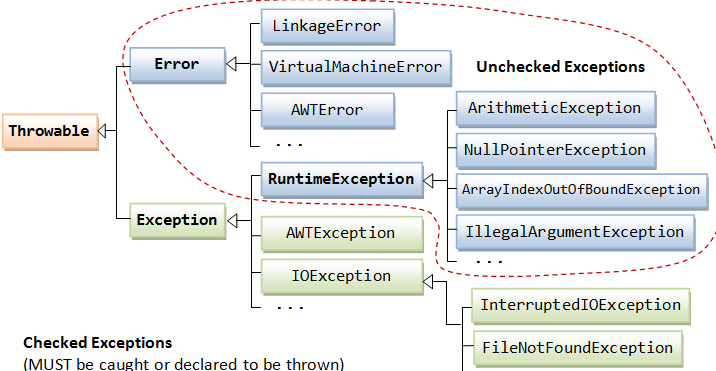
\includegraphics[width=%
0.6\textwidth]{eccezioni}
\end{center} 
\newpage









\newpage
\section{21-03-2019: COLLECTION, LIST E SET}
\begin{center}
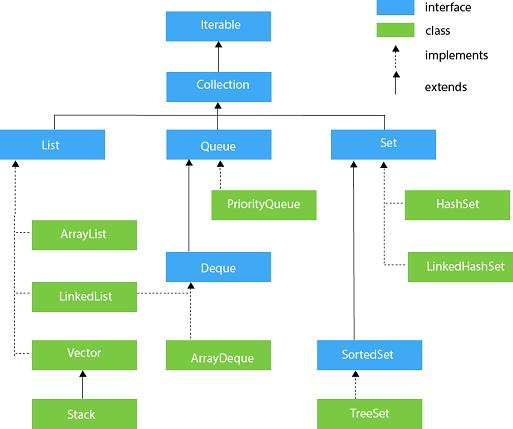
\includegraphics[width=%
0.6\textwidth]{java-collection-hierarchy}
\end{center} 

\begin{center}
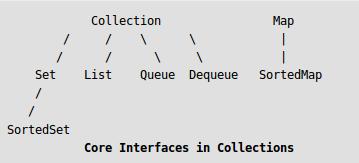
\includegraphics[width=%
0.6\textwidth]{MapInterface}
\end{center} 
\textbullet\ -> ITERABLE:Posso solo scorrere \newline
\textbullet\ ---> COLLECTION: Posso scorrere, aggiungere e togliere \newline
\textbullet\ -----> LIST: Posso scorrere e aggiungere o togliere con un indice \newline
\textbullet\ -------> ARRAYLIST:è sottotipo di list, in quanto implementa list! \newline
\digraph{ao}{rankdir=LR;

   a [label="Iterable" shape = "record"]; 
   b [label="Collection" shape = "record"]; 
   c [label="Set" shape = "record"]; 
   d [label="Hash" shape = "record"]; 
   e [label="List" shape = "record"]; 
   f [label="ArrayList" shape = "record"];    
   b->a; e->b; f->e; d->c; c->b} \newline

\noindent Per evitare di riprodurre codice si usano le classi astratte dalle quali poi si erediterà. 

\noindent Relazione di ordinamento: operatore binario che permette di mappare elementi di due insiemi diversi.

\noindent Una classe con metodi tutti statici non si può costruire. Rappresenta dunque un contenitore di metodi (è un pezzo di libreria).

\noindent \textbf{CARATTERISTICHE DI SET}\newline
\textbullet\ Gli elementi non sono duplicati \newline
\textbullet\ Gli elementi non sono ordinati in base a come sono inseriti \newline	
\textbullet\ Non vengono inseriti metodi nuovi, eredita solo quelli del padre \newline
\textbullet\ I metodi nuovi vengono messi nella classe che implementa l'interfaccia \newline
\textbullet\ Tiene un ordinamento che cerca di massimizzare le operazioni di ricerca ed estrazione \newline

\noindent \textbf{CARATTERISTICHE DI LIST}\newline
\textbullet\ Gli elementi possono essere duplicati \newline
\textbullet\ Gli elementi sono ordinati in base all'ordine di inserimento \newline	
\textbullet\ Rispetto ai metodi del padre ne aggiunge altri che permettono di leggere ed inserire elementi in un determinato indice \newline

\noindent \textbf{CODICE DI ESEMPIO}\newline
Il professore questo giorno ha caricato su github del codice chiamato: TinyJDK. Lo riporto per completezza:
\begin{lstlisting}[basicstyle=\small,]
/* Classe: MyIterable.java */
public interface MyIterable<E> {

    MyIterator<E> iterator();
    int find(E x) throws Exception;

}
\end{lstlisting}

\begin{lstlisting}[basicstyle=\small,]
/* Classe: MyIterator.java */
public interface MyIterator<E> {
    boolean hasNext();
    E next();
}
\end{lstlisting}

\begin{lstlisting}[basicstyle=\small,]
/* Classe: MyCollection.java */
import java.util.Collection;
import java.util.function.Function;

public interface MyCollection<T> extends MyIterable<T> {
    void add(T x);
    void clear();
    void remove(T x);   // da decidere se ci piace o no
    boolean contains(T x);
    boolean contains(Function<T, Boolean> p);
    int size();


}
\end{lstlisting}

\begin{lstlisting}[basicstyle=\small,]
/* Classe: MyList.java */

public interface MyList<T> extends MyCollection<T> {
    void add(int i, T x);
    T get(int i);
    void set(int i, T x);
}
\end{lstlisting}

\begin{lstlisting}[basicstyle=\small,]
/* Classe: MySet.java */
public interface MySet<T> extends MyCollection<T> {
}
\end{lstlisting}

\noindent \textbf{ESEMPIO IMPLEMENTAZIONE LIST}\newline
Vediamo un esempio di implementazione della classe List, collection in cui gli elementi vengono memorizzati in ordine di arrivo.

\begin{lstlisting}[basicstyle=\small,]
/* Classe: MyArrayList.java */
import java.util.Collection;
import java.util.function.Function;

public class MyArrayList<T> implements MyList<T> {

    private Object[] a;
    private int actualSize;

    public static class MyException extends Exception {
        public MyException(String s) {
            super(s);
        }
    }

/*    T[] toArray() {
        return (T[]) a;
    }*/

/*    public static Exception returnNow() {
        return new Exception("msg");
    }

    public static void throwNow() throws Exception {
        throw new Exception("msg");
    }

    public static void caller() throws Exception {
        Exception e = returnNow();
        throwNow();
    }

    public static void caller2() {
        try {
            caller();
        }
        catch (Exception e2) {
            // fai qualcosa con e2
        }

    }

    public void m(int x) throws Exception {
        MyException e = new MyException("error messagge");
        if (x < 0) throw e;
    }
  */

    public MyArrayList() {
        clear();
    }

    public static class NotFoundException extends Exception {
    }

	/* ritorna l'indice in cui è memorizzato un oggetto equivalente a 
	 * quello passato come parametro di ingresso */
    @Override
    public int find(T x) throws NotFoundException {
        int cnt = 0;
        MyIterator<T> it = iterator();
        while (it.hasNext())
        {
            T y = it.next();
            if (x.equals(y)) return cnt;
            ++cnt;
        }
        throw new NotFoundException();
    }




    public static void main3() {
        MyArrayList<Integer> c = new MyArrayList<>();
        try {
            int index = c.find(6);
            System.out.println("found at index = " + index);
        } catch (NotFoundException e) {
            try {
                int index = c.find(7);
            } catch (NotFoundException e1) {

            }

        }
    }

    @Override
    public boolean contains(T x) {
        for (int i = 0; i < actualSize; ++i) {
            Object o = a[i];
            if (o.equals(x)) return true;
        }
        return false;
    }


    @Override
    public boolean contains(Function<T, Boolean> p) {
        return false;
    }

    @Override
    public int size() {
        return actualSize;
    }


    @Override
    public void clear() {
        a = new Object[100];
        actualSize = 0;
    }

    @Override
    public void add(T o) {
        a[actualSize++] = o;
        if (actualSize >= a.length) {
            Object[] u = new Object[a.length * 2];
            for (int j = 0; j < a.length; ++j)
                u[j] = a[j];
            a = u;
        }
    }

    @Override
    public MyIterator<T> iterator() {
        return new MyIterator<T>() {
            private int pos = 0;

            @Override
            public boolean hasNext() {
                return pos <= actualSize;
            }

            @Override
            public T next() {
                return (T) MyArrayList.this.a[pos++];
            }
        };
    }

    @Override
    public void add(int i, T x) {

    }

    @Override
    public T get(int i) {
        return (T) a[i];
    }

    @Override
    public void set(int i, T x) {
        a[i] = x;
    }

    @Override
    public void remove(T x) {

    }

}
\end{lstlisting}

\noindent \textbf{ESEMPIO IMPLEMENTAZIONE SET}\newline
Vediamo un esempio di implementazione della classe Set, collection in cui gli elementi vengono inseriti secondo una certa logica interna. In questo caso gli elementi verranno tenuti secondo l'ordine imposto o da comparator o da comparable.

\begin{lstlisting}[basicstyle=\small,]
/* Classe: MyArrayListSet.java */
import java.util.ArrayList;
import java.util.Arrays;
import java.util.Collections;
import java.util.Comparator;
import java.util.function.Function;

public class MyArrayListSet<T extends Comparable<T>> implements MySet<T> {
    private final Comparator<T> p;
    private final ArrayList<T> a;

    public MyArrayListSet(Comparator<T> p) {
        this.a = new ArrayList<T>();
        this.p = p;
    }

    @Override
    public void add(T x) {
        if (!contains(x)) {
            a.add(x);
            sort();
        }
    }

    private void sort() {
        Collections.sort(a, p);
    }

    @Override
    public void clear() {
        a.clear();
    }

    @Override
    public void remove(T x) {
        a.remove(x);
    }

    @Override
    public boolean contains(T x) {
        return a.contains(x);
    }

    @Override
    public boolean contains(Function<T, Boolean> p) {
        return a.contains(p);
    }

    @Override
    public int size() {
        return a.size();
    }

    @Override
    public MyIterator<T> iterator() {
        return a.iterator();
    }

    @Override
    public int find(T x) throws Exception {
        return a.find(x);
    }
}
\end{lstlisting}








\newpage
\section{25-03-2019}
\noindent Ha continuato quello che ha fatto la scorsa lezione \newline
Inserisco il codice caricato dal professore quel giorno, esso o modifica classi già definite la lezione precedente o ne aggiunge di nuove: 

\begin{lstlisting}[basicstyle=\small,]
/* Classe: MySortedSet.java */
public interface MySortedSet<T extends Comparable<T>> extends MySet<T> {

}
\end{lstlisting}

\begin{lstlisting}[basicstyle=\small,]
/* Classe: MyArrayListSortedSet.java */
import java.util.*;
import java.util.function.Function;

public class MyArrayListSortedSet<T extends Comparable<T>>
        extends MyAbstractArrayListSet<T> {

    public MyArrayListSortedSet() {
        super();
    }

    @Override
    protected void sort() {
        Collections.sort(a);
    }

}
\end{lstlisting}

\begin{lstlisting}[basicstyle=\small,]
/* Classe: MyArrayListSet.java */
/* è stata modificata la classe dell'altra volta*/

import java.util.*;
import java.util.function.Function;

public class MyArrayListSet<T> extends MyAbstractArrayListSet<T> {

    private final Comparator<T> p;

    public MyArrayListSet(Comparator<T> p) {
        super();
        this.p = p;
    }

    @Override
    protected void sort() {
        Collections.sort(a, p);
    }

}

\end{lstlisting}

\begin{lstlisting}[basicstyle=\small,]
/* Classe: MyAbstractArrayListSet.java */
import java.util.*;
import java.util.function.Function;

public abstract class MyAbstractArrayListSet<T> implements MySet<T> {
    protected final ArrayList<T> a;

    protected MyAbstractArrayListSet() {
        this.a = new ArrayList<T>();
    }

    @Override
    public void add(T x) {
        if (!contains(x)) {
            a.add(x);
            sort();
        }
    }

    protected abstract void sort();

    @Override
    public void clear() {
        a.clear();
    }

    @Override
    public void remove(T x) {
        a.remove(x);
    }

    @Override
    public boolean contains(T x) {
        return a.contains(x);
    }

    @Override
    public boolean contains(Function<T, Boolean> p) {
        return a.contains(p);
    }

    @Override
    public int size() {
        return a.size();
    }

    @Override
    public MyIterator<T> iterator() {
        Iterator<T> it = a.iterator();
        return new MyIterator<T>() {

            @Override
            public boolean hasNext() {
                return it.hasNext();
            }

            @Override
            public T next() {
                return it.next();
            }
        };
    }

    @Override
    public int find(T x) throws Exception {
        int r = a.indexOf(x);
        if (r < 0) throw new Exception("not found");
        return r;
    }
}

\end{lstlisting}

\begin{lstlisting}[basicstyle=\small,]
/* Classe: Main.java */
import java.util.*;

public class Main {

    public static class Plant {
        private int height;

    }

    public static class Animal implements Comparable<Animal> {
        private int weight;
        private String name;

        public Animal(String name, int w) {
            this.name = name;
            this.weight = w;
        }

        public int getWeight() { return weight; }

        public String getName() {
            return name;
        }

        @Override
        public int compareTo(Animal o) {
            return this.weight - o.weight;
            /*if (this.weight == o.weight) return 0;
            else if (this.weight > o.weight) return 1;
            else return -1;*/
        }
    }

    public static class Dog extends Animal {

        public Dog(String name, int w) {
            super(name, w);
        }
    }

    public static void main(String[] args) {

        List<Animal> a = new ArrayList<>();
        Collections.sort(a);

        List<Plant> b = new ArrayList<>();
        Collections.sort(b, new Comparator<Plant>() {
            @Override
            public int compare(Plant x, Plant y) {
                return x.height - y.height;
            }
        });

    }
}
\end{lstlisting}


\newpage
\section{28-03-2019}
\noindent Affinchè due classi siano confrontabili devono implementare il metodo compare to \newline
Solitamente si usa il modificatore protected invece che private in modo tale che da fuori non possano essere modificate, ma possano essere viste quando vengono ereditate. \newline

\noindent \textbf{MAPPE}\newline
Una mappa è un oggetto che mappa chiavi con valori. Non ci possono essere chiavi duplicate e ogni chiave può mappare al più un valore. \newline
Una mappa rappresenta una collection associativa. \newline
Una mappa è parametrica su due tipi di argomenti. Uno rappresenta il dominio (chiave), e l'altro rappresenta il codominio (valore). La gerarchia delle mappe è slegata dalla gerarchia delle collection. \newline
Per la documentazione java sulle mappe consultare questo \href{https://docs.oracle.com/javase/8/docs/api/java/util/Map.html }{SITO} \newline
Una mappa è una collection associativa, con coppie associate a valori.

\noindent Il foreach di JAVA funziona solo con le librerie del JDK originale di JAVA.\newline
Super può essere usato per il costruttore o per metodi che eredito, non è di perse un metodo e non ha un tipo.

\noindent Durante la lezione il professore ha aggiunto nel repository di github il seguente codice: 


\begin{lstlisting}[basicstyle=\small,]
/* Classe: Pair.java */
public class Pair<A, B> {
    private A a;
    private B b;

    public Pair(A a, B b) {
        this.a = a;
        this.b = b;
    }

    public A getFirst() { return a; }
    public B getSecond() { return b; }

}
\end{lstlisting}

\begin{lstlisting}[basicstyle=\small,]
/* Classe: NotFoundException.java */
public class NotFoundException extends Exception {
}
\end{lstlisting}

\begin{lstlisting}[basicstyle=\small,]
/* Classe: MyMap.java */
public interface MyMap<K, V> extends MyCollection<Pair<K, V>> {
	/*K = sono le chiavi */
	/*V = sono i valori  */
    void put(K key, V value);
    V get(K key) throws NotFoundException;

}
\end{lstlisting}

\noindent Decidiamo di implementare la nostra mappa in due maniere diverse! 

\begin{lstlisting}[basicstyle=\small,]
/* Classe: MyListMap__old.java */
import java.util.function.Function;

public class MyListMap__old<K, V> implements MyMap<K, V> {

    private MyList<Pair<K, V>> l;

    public MyListMap__old() {
        this.l = new MyArrayList<>();
    }

    @Override
    public void put(K key, V value) {
        l.add(new Pair<K, V>(key, value));
    }

    @Override
    public V get(K key) throws NotFoundException {
        MyIterator<Pair<K, V>> it = l.iterator();
        while (it.hasNext()) {
            Pair<K, V> p = it.next();
            if (key.equals(p.getFirst())) return p.getSecond();
        }
        throw new NotFoundException();
    }

    @Override
    public void add(Pair<K, V> x) {
        put(x.getFirst(), x.getSecond());
    }

    @Override
    public void clear() {
        l.clear();
    }

    @Override
    public void remove(Pair<K, V> x) {
        l.remove(x);
    }

    @Override
    public boolean contains(Pair<K, V> x) {
        return l.contains(x);
    }

    @Override
    public boolean contains(Function<Pair<K, V>, Boolean> p) {
        return l.contains(p);
    }

    @Override
    public int size() {
        return l.size();
    }

    @Override
    public MyIterator<Pair<K, V>> iterator() {
        return l.iterator();
    }

    @Override
    public int find(Pair<K, V> x) throws Exception {
        return l.find(x);
    }
}
\end{lstlisting}

\begin{lstlisting}[basicstyle=\small,]
/* Classe: MyListMap.java */
public class MyListMap<K, V> extends MyArrayList<Pair<K, V>>
        implements MyMap<K, V> {

    @Override
    public void put(K key, V value) {
        add(new Pair<K, V>(key, value));
    }

    @Override
    public V get(K key) throws NotFoundException {
        MyIterator<Pair<K, V>> it = iterator();
        while (it.hasNext()) {
            Pair<K, V> p = it.next();
            if (key.equals(p.getFirst())) return p.getSecond();
        }
        throw new NotFoundException();
    }
}
\end{lstlisting}

\begin{lstlisting}[basicstyle=\small,]
/* Classe: MyArrayListSortedSet.java */
/* è stata modificata la classe dell'altra volta*/
import java.util.*;
import java.util.function.Function;

public class MyArrayListSortedSet<T extends Comparable<T>>
        extends MyAbstractArrayListSet<T>
        implements MySortedSet<T> {

    public MyArrayListSortedSet() {
        super();
    }

    @Override
    protected void sort() {
        Collections.sort(a);
    }

}
\end{lstlisting}

\begin{lstlisting}[basicstyle=\small,]
/* Classe: MyArrayList.java */
/* è stata modificata la classe dell'altra volta*/
import java.util.function.Function;

public class MyArrayList<T> implements MyList<T> {

    private Object[] a;
    private int actualSize;

    public static class MyException extends Exception {
        public MyException(String s) {
            super(s);
        }
    }

/*    T[] toArray() {
        return (T[]) a;
    }*/

/*    public static Exception returnNow() {
        return new Exception("msg");
    }

    public static void throwNow() throws Exception {
        throw new Exception("msg");
    }

    public static void caller() throws Exception {
        Exception e = returnNow();
        throwNow();
    }

    public static void caller2() {
        try {
            caller();
        }
        catch (Exception e2) {
            // fai qualcosa con e2
        }

    }

    public void m(int x) throws Exception {
        MyException e = new MyException("error messagge");
        if (x < 0) throw e;
    }
  */

    public MyArrayList() {
        clear();
    }

    @Override
    public int find(T x) throws NotFoundException {
        int cnt = 0;
        MyIterator<T> it = iterator();
        while (it.hasNext())
        {
            T y = it.next();
            if (x.equals(y)) return cnt;
            ++cnt;
        }
        throw new NotFoundException();
    }




    public static void main3() {
        MyArrayList<Integer> c = new MyArrayList<>();
        try {
            int index = c.find(6);
            System.out.println("found at index = " + index);
        } catch (NotFoundException e) {
            try {
                int index = c.find(7);
            } catch (NotFoundException e1) {

            }

        }
    }

    @Override
    public boolean contains(T x) {
        for (int i = 0; i < actualSize; ++i) {
            Object o = a[i];
            if (o.equals(x)) return true;
        }
        return false;
    }


    @Override
    public boolean contains(Function<T, Boolean> p) {
        return false;
    }

    @Override
    public int size() {
        return actualSize;
    }


    @Override
    public void clear() {
        a = new Object[100];
        actualSize = 0;
    }

    @Override
    public void add(T o) {
        a[actualSize++] = o;
        if (actualSize >= a.length) {
            Object[] u = new Object[a.length * 2];
            for (int j = 0; j < a.length; ++j)
                u[j] = a[j];
            a = u;
        }
    }

    @Override
    public MyIterator<T> iterator() {
        return new MyIterator<T>() {
            private int pos = 0;

            @Override
            public boolean hasNext() {
                return pos <= actualSize;
            }

            @Override
            public T next() {
                return (T) MyArrayList.this.a[pos++];
            }
        };
    }

    @Override
    public void add(int i, T x) {

    }

    @Override
    public T get(int i) {
        return (T) a[i];
    }

    @Override
    public void set(int i, T x) {
        a[i] = x;
    }

    @Override
    public void remove(T x) {

    }

}

\end{lstlisting}

\begin{lstlisting}[basicstyle=\small,]
/* Classe: Main.java */
/* è stata modificata la classe dell'altra volta*/
import java.util.*;

public class Main {

    public static class Plant {
        private int height;

    }

    public static class Animal implements Comparable<Animal> {
        private int weight;
        private String name;

        public Animal(String name, int w) {
            this.name = name;
            this.weight = w;
        }

        public int getWeight() { return weight; }

        public String getName() {
            return name;
        }

        @Override
        public int compareTo(Animal o) {
            return this.weight - o.weight;
            /*if (this.weight == o.weight) return 0;
            else if (this.weight > o.weight) return 1;
            else return -1;*/
        }
    }

    public static class Dog extends Animal {

        public Dog(String name, int w) {
            super(name, w);
        }
    }


    public static void main2() {
        MyCollection<Pair<String, Integer>> rubrica = new MyListMap<>();
        rubrica.add(new Pair<>("Alvise", 34712345));
        rubrica.add(new Pair<>("Diego", 987654321));
    }


    public static void main(String[] args) {

        List<Animal> a = new ArrayList<>();
        Collections.sort(a);

        List<Plant> b = new ArrayList<>();
        Collections.sort(b, new Comparator<Plant>() {
            @Override
            public int compare(Plant x, Plant y) {
                return x.height - y.height;
            }
        });

    }
}
\end{lstlisting}

\noindent Finita la lezione il professore ha deprecato la classe: MyListMap\_ \_ old.java


\newpage
\section{1-04-2019: HASH MAP}
\textbf{HASH MAP} \newline
Le hash Map sono sempre delle mappe, solo che il tipo di una chiave viene identificato con un interno. Questo può rendere a ricerca più veloce!. \newline
Per cercare si esegue l'hash di quello che voglio cercare (per esempio hashare una stringa), poi vado a cercare in un array indicizzato ( questa operazione costa O(1) costante). \newline
Le l'hash map sono però inefficienti in termini di memoria. 

\noindent Il costruttore dell' hash map è il seguente: 
\begin{lstlisting}[basicstyle=\small,]
	HashMap(int initalcapacity, float loadFactor)
\end{lstlisting}
Esso costruisce una hash map vuota con una capacità iniziale uguale a quella specificatta e con un fattore di carico. Il fattore di carico (load factor) specifica di quanto si deve moltiplicare quando si ingrandisce la mappa. 
\begin{lstlisting}[basicstyle=\small,]
	HashMap(Map<? extends k, ? extends v> m)
\end{lstlisting}
Costruisce una nuova hash map, popolandola con i valori della mappa passata. Viene chiamato costruttore per copia.

\noindent Si subsume fino al punto che serve (un buon compromesso è subsumere fino all'interfaccia). Se però mi servono dei metodi specifici, non possono subsumere. 

\noindent La classe Object ha un metodo hashcode che tutti gli oggetti ereditano. Serve per hashare this.



\noindent Il professore ha aggiunto il seguente codice nel suo repository github quel giorno: 

\begin{lstlisting}[basicstyle=\small,]
/* Classe: Main.java */
/* è stata modificata la classe dell'altra volta */
/* Ha aggiunto solo l'hashCode e il main3()      */

import java.util.*;

public class Main {

    public static class Plant {
        private int height;

    }

    public static class Animal implements Comparable<Animal> {
        private int weight;
        private String name;

        public Animal(String name, int w) {
            this.name = name;
            this.weight = w;
        }

        public int getWeight() { return weight; }

        public String getName() {
            return name;
        }

        @Override
        public int compareTo(Animal o) {
            return this.weight - o.weight;
        }

        @Override
        public int hashCode() {
            return weight * name.hashCode();
        }

    }

    public static class Dog extends Animal {

        public Dog(String name, int w) {
            super(name, w);
        }

        @Override
        public int hashCode() {
            return super.hashCode();
        }
    }

    public static void main3() {

        Map<Dog, String> m = new HashMap<>();
        Dog emma = new Dog("emma", 10);
        Dog toby = new Dog("toby", 10);
        Dog bob = new Dog("bob", 20);

        m.put(emma, "cecilia");
        m.put(toby, "mihail");
        m.put(bob, "alex");
    }





    public static void main2() {
        MyCollection<Pair<String, Integer>> rubrica = new MyListMap<>();
        rubrica.add(new Pair<>("Alvise", 34712345));
        rubrica.add(new Pair<>("Diego", 987654321));
    }


    public static void main(String[] args) {

        List<Animal> a = new ArrayList<>();
        Collections.sort(a);

        List<Plant> b = new ArrayList<>();
        Collections.sort(b, new Comparator<Plant>() {
            @Override
            public int compare(Plant x, Plant y) {
                return x.height - y.height;
            }
        });

    }
}


\end{lstlisting}
 





\newpage
\section{4-04-2019: SINGLETON E THREAD}
\textbf{DESIGN PATTERN SINGLETON} \newline
Si limita l'istanzazione di una classe a una sola istanza. \newline
Può servire per creare oggetti statici (per esempio un campo statico esiste anche prima dell'istanza dell'oggetto del tipo della classe a cui appartiene). \newline
Un costruttore privato può essere accessibile solo dalla classe, e non dall'esterno. \newline
I metodi statici che ritornano lo stesso tipo del costruttore della classe sono costruttori travestiti. \newline
i costruttori sono metodi d'istanza. Non serve il modificatore di accesso static, anche se sono simili a metodi statici. \newline
I metodi statici sono pseudo costruttori, se usati nel modo opportuno. \newline
Un metodo statico è un metodo che non ha bisogno di istanza. Un campo statico si può vedere anche se non ha istanza (da un metodo statico si può accedere solo a campi statici, poichè non ha riferimento al this). \newline
In questo corso non andremo oltre con questo design pattner perchè sempre di più in programmazione si sta andando verso la programmazione funzionale (in contrapposizione a quella imperattiva).


\begin{lstlisting}[basicstyle=\small,]
/* Classe: Main.java */
package patterns.singleton;

public class Main {

    public static void main(String[] args) {
        Singleton single1 = Singleton.getInstance();
        Singleton single2 = Singleton.getInstance();
        System.out.println("is it the same object? " + (single1 == single2));
    }

}

\end{lstlisting}

\begin{lstlisting}[basicstyle=\small,]
/* Classe: Singleton.java */
package patterns.singleton;

class Singleton {
    private static Singleton instance = null;

    // costruttore privato per non permettere a nessuno di costruire questa classe
    private Singleton() {}

    // metodo statico che funge da pseudo-costruttore
    public static Singleton getInstance() {
        if (instance == null)
            instance = new Singleton();
        return instance;
    }
}

\end{lstlisting}


\noindent \textbf{INTERFACCIA GRAFICA} \newline
Un widget è un supertipo dell'interfaccia grafica. \newline
Busy-Loop: ciclo che cicla a vuoto, non restituendo il controllo al S.O. \newline
Le interfacce grafiche non si programmano a busy-loop. Si chiede al sistema operativo di "svegliarmi quando accade un evento". Dunque si programmano a suon di call-back. \newline
Un esempio di call-back è il ctr-c per interrompere un programma in una shell linux. Questa combinazione di tasti manda un segnale, ma in realtà viene invocata una call-back. \newline
Programmazion ad eventi: si programma con la call-back che vengono chaimate quando opportuno.

\noindent \textbf{THREAD IN JAVA} \newline
Per generare dei \textit{Thread} in java esistono principalmente due metodi: \newline
\textbullet\ Si estende la classe \textit{Thread} e si fa l'override del metodo \textit{run} \newline
\textbullet\ Si istanzia la classe \textit{Thread} passando al costruttore un istanza di una classe che implementa l'interfaccia \textit{Runnable}



\begin{lstlisting}[basicstyle=\small,]
/* Classe: Main.java */
package threads;

public class Main {

    private static void loop(int n, int ms) {
        for (int i = 0; i < n; ++i) {
            System.out.println(String.format("thread[%d]: #%d", Thread.currentThread().getId(), i));
            try {
                Thread.sleep(ms);
            } catch (InterruptedException e) {
                e.printStackTrace();
            }
        }
    }

    public static class MyThread extends Thread {
        private final int n;

        public MyThread(int n) {
            this.n = n;
        }

        @Override
        public void run() {
            Main.loop(n, 300);
        }

    }


    public static void main(String[] args) {
        MyThread th = new MyThread(23);
        /* thread start comincia un nuovo thread
         * e poi invoca il run */
        th.start();
        
        /* Richiamare il run cosi avvia semplicemente 
         * il metodo run, ma senza cominciare un nuovo 
         * thread. infatti le chiamate di questo run
         * si sovrappongono a quelle dello start */
        th.run();
        
        /* Questa procedura parte dopo che è stata 
         * richiamata e terminata quella invocata
         * da th.run() */
        loop(11, 500);
    }

}
\end{lstlisting}

\noindent \textbf{SLEEP} \newline
Thread.sleep è un metodo che lancia una checked exception (eccezione a gestione obbligatoria), quindi bisogna sempre metterlo all'interno di un try catch, pena un errore in compilazione. Ma perchè? se un'altro thread richiama sul nostro thread che sta dormendo la funzione: \textit{interrupt()} il thread verrà risvegliato e verrà lanciata da esso l'eccezione \textit{InterruptedException}
 

 



\newpage
\section{8-04-2019}
\noindent Non ho ancora messo apposto gli appunti di quel giorno però intanto importo il codice scritto dal professore: 

THREAD

\begin{lstlisting}[basicstyle=\small,]
/* Classe: Main.java */
package threads;

public class Main {

    private static void loop(int n, int ms) {
        for (int i = 0; i < n; ++i) {
            System.out.println(String.format("thread[%d]: #%d", Thread.currentThread().getId(), i));
            try {
                Thread.sleep(ms);
            } catch (InterruptedException e) {
                e.printStackTrace();
            }
        }
    }

    public static class MyThread extends Thread {
        private final int n;

        public MyThread(int n) {
            this.n = n;
        }

        @Override
        public void run() {
            Main.loop(n, 300);
        }

    }


    public static void main(String[] args) {
        MyThread th = new MyThread(23);
        th.start();
        th.run();
        loop(11, 500);
    }

}


\end{lstlisting}

 
SINGLETON
 
\begin{lstlisting}[basicstyle=\small,]
/* Classe: Main.java */
package patterns.singleton;

public class Main {

    public static void main(String[] args) {
        Singleton single1 = Singleton.getInstance();
        Singleton single2 = Singleton.getInstance();
        System.out.println("is it the same object? " + (single1 == single2));
    }

}

\end{lstlisting}

\begin{lstlisting}[basicstyle=\small,]
/* Classe: Singleton.java */
package patterns.singleton;

class Singleton {
    private static Singleton instance = null;

    // costruttore privato per non permettere a nessuno di costruire questa classe
    private Singleton() {}

    // metodo statico che funge da pseudo-costruttore
    public static Singleton getInstance() {
        if (instance == null)
            instance = new Singleton();
        return instance;
    }
}

\end{lstlisting}


\newpage
\section{11-04-2019: THREAD POOL}
\noindent Gli appunti dell'altra volta sono gli stessi di questa lezione, il professore ha aggiunto un po di codice.
 


\begin{lstlisting}[basicstyle=\small,]
/* Classe: SynchronizedMain.java */
/* ha modificato il codice della scorsa volta */
/* riporto solo la modifica */
    public static void main(String[] args) {
//        MyThread th = new MyThread(500);
//        th.start();
        new MyThread(500).start();

        new Thread(() -> loop(400)).start();

        loop(300);
    }
\end{lstlisting}

\noindent Sucecssivamente è tornato a concentrarsi sui thread pool.

\begin{lstlisting}[basicstyle=\small,]
/* Classe: ThreadPool.java */
package threads;

public class ThreadPool implements Queue<Thread> {



}

\end{lstlisting}

\begin{lstlisting}[basicstyle=\small,]
/* Classe: ThreadPool.java */
import java.util.Queue;
import java.util.concurrent.ConcurrentLinkedQueue;

public class ThreadPool {
    private Queue<PooledThread> q = new ConcurrentLinkedQueue<>();

    public static class PooledThread extends Thread {
        private Runnable r;
    }

    public PooledThread acquire(Runnable cb) {
        if (q.isEmpty()) {
            return new PooledThread();
        }
        else {
            PooledThread p = q.poll();
            p.notify();
        }
    }

    public void release(PooledThread t) {
        q.add(t);
    }

    public static void threadMain(PooledThread p) {
        while (true) {
            try {
                p.wait();
                p.r.run();  // TODO: potrebbe essere null
            } catch (InterruptedException e) {
                e.printStackTrace();
            }
        }
    }

    public static void main(String[] args) {
        ThreadPool pool = new ThreadPool();
        Thread t1 = pool.acquire();
        t1.
    }
}


\end{lstlisting}




\noindent Sucecssivamente ha modificato ancora la synconized main

\begin{lstlisting}[basicstyle=\small,]
/* Classe: SynchronizedMain.java */
/* è stata modificata la classe di prima    */
/* ne riporto solamente la modifica al main */
    public static void main(String[] args) {
        MyThread th1 = new MyThread(500);
        th1.start();    // spawn thread 1

        // non serve conservare l'oggetto thread in una variabile se non è necessario
        new Thread(() -> loop(400)).start();    // spawn thread 2 con un runnable in costruzione

        // esegue lo stesso codice anche col main thread
        loop(300);  
    }

\end{lstlisting}













\newpage
\section{15-04-2019}
\noindent PLACE HOLDER
 





\newpage
\section{18-04-2019: THREAD POOL}
\noindent \textbf{CONTINUAZIONE DEI THREAD} \newline
Thread.currentThread() ritorna un oggetto di tipo thread che rappresenta se stesso. Ritorna una istanza della classe Thread in carica di eseguire il thread. \newline
Il metodo run non può lanciare nessuna eccezione di tipo checked \newline
Quando si usano i timeout si è soliti specificare quanto tempo e l'unità di misura. Essa si può specificare usando TimeUnit.UNITADIMISURA. \newline

\noindent \textbf{ESPRESSIONI LAMBDA} \newline
Sintassi: \newline
\textbullet\ $ (\tau_{1} x_{1} , .... , \tau_{n} x_{n}) -> E $ Dove E è un'espressione \newline
Vengono passati anche i tipi in quanto non c'è un type inference completo. Inoltre l'espressione della lambda può essere anche un blocco. \newline
Vediamo degli esempi: \newline
\textbullet\ $ (int n) -> (n+1) $ E' corretta \newline
\textbullet\ $ (int x) -> return x+1 $ E' errata. infatti il return non è un'espressione, è uno statament, dunque ci vanno le graffe. \newline
\textbullet\ $ (int x) -> {return x+1} $ E' corretta \newline
\textbullet\ $ () -> 1 $ E' corretta \newline
In generale se l'espressione lambda è semplice si possono omettere le graffe, mentre se ha uno statament bisogna metterci le graffe. \newline


\noindent \textbf{CODICE DEL PROFESSORE} \newline
\begin{lstlisting}
/* Classe: ThreadPool.java */
/* Ha modificato la classe che
 * stava in work.
 * ha tolto lo static dalla classe
 * PooledThread ed ha aggiunto un 
 * q.add(this)*/
package threads.work_in_progress;

import org.jetbrains.annotations.NotNull;
import org.jetbrains.annotations.Nullable;

import java.util.Objects;
import java.util.Queue;
import java.util.concurrent.ConcurrentLinkedQueue;

public class ThreadPool {
    private Queue<PooledThread> q = new ConcurrentLinkedQueue<>();

    public class PooledThread extends Thread {
        @Nullable
        private Runnable currentRunnable;

        @Override
        public void run() {
            while (true) {
                try {
                    synchronized (this) {
                        print("waiting...");
                        wait();
                        print("awaken");
                    }
                    Objects.requireNonNull(currentRunnable).run();
                    print("requeueing");
                    q.add(this);
                } catch (InterruptedException e) {
                    e.printStackTrace();
                }
            }
        }

        @Override
        public String toString() {
            return String.format("[%s:%d]", this.getName(), this.getId());
        }

    }

    public PooledThread acquire(Runnable cb) {
        @NotNull final PooledThread p;
        if (q.isEmpty()) {
            print("spawning");
            p = new PooledThread();
            p.start();
        } else {
            p = q.poll();
        }
        print("notify");
        synchronized (p) {
            p.currentRunnable = cb;
            p.notify();
            return p;
        }
    }

    public static void main(String[] args) {
        ThreadPool pool = new ThreadPool();
        Thread t1 = pool.acquire(() -> {
            try {
                Thread.sleep(300);
            } catch (InterruptedException e) {
                e.printStackTrace();
            }
            print("bye");
        });
    }

    private static void print(String s) {
        System.out.println(String.format("%s: %s", Thread.currentThread(), s));
    }
}

\end{lstlisting}
 





\newpage
\section{29-04-2019: PRODUTTORE CONSUMATORE}

\noindent \textbf{DESIGN PATTNER: PRODUTTORE CONSUMATORE} \newline
La filosofia è questa: qualcuno produce le cose e qualcun altro le utilizza. Ad esempio un thread produce i dati mettendoli in una coda ed un'altro thread li consuma estraendoli. \newline
Rilassare un'eccezione significa salire di livello nella gerarchia. Invece che raccogliere un'eccezione specifica le raccolgo tutte, ad esempio usando: catch(Exception e). \newline
Le stringhe in java non sono mutabili. \newline
Tutte le strutture che implementano cose bloccanti sono anche thread safe. \newline
Un oggetto non viene preso in carico dal garbage collector quando è dentro una variabile e quando è dentro ad una struttura dati. Questo, se non si presta attenzione, può portare al fenomeno della memory leak (ingrossamento della memoria a dismisura). \newline

\noindent \textbf{CODE BLOCCANTI} \newline
Per trattare il tema produttore consumatore andremo ad utilizzare delle code bloccanti. Questo perchè abbiamo due problemi: il primo è che non possiamo aggiungere dati alla coda se essa è piena, il secondo è che non possiamo retribuire dati da una coda se essa è vuota. Le code bloccanti risolvono questi problemi esportando le seguenti api: \newline
\textbullet\ put(): inserisce un elemento nella coda aspettando che ci sia uno slot libero. \newline
\textbullet\ add(): inserisce un elemento nella coda e ritorna true, se non riesce ad inserirlo (coda piena) ritorna false. \newline
\textbullet\ take(): prende un elemento dalla testa della coda aspettando, in maniera bloccante, che la coda non sia vuota. \newline
\textbullet\ poll(timeout): prende un elemento dalla testa della coda aspettando, per un certo timeout.\newline

\noindent \textbf{CODE BLOCCANTI VS NON } \newline
Abbiamo già visto un esempio di coda non bloccante: ConcurrentLinkedQueue \newline
La differenza tra le due è che una blocca le richieste di inserimento ed accesso ai dati, aspettando che le condizioni necessarie vengano soddisfatte, mentre l'altra ritorna false nel caso non riuscisse a svolgere subito le sue operazioni.\newline

\noindent \textbf{CLASSE RANDOM } \newline
La classe Random ci aiuta a generare numeri casuali in Java. Essa possiede due costruttori, uno vuoto ed uno che prende come parametro un tipo intero long. Visto che le i generatori di numeri casuali non producono effettivamente numeri veramente casuali impostare un certo seed ci permette di settare lo stato iniziale del generatore di numeri casuali. Dati due generatori Random con lo stesso stato iniziale (o quindi lo stesso seed) otterremo in uscita una sequenza di numeri identica.
\begin{lstlisting}
/* Sceglie un seed casuale */
public Random();
/* Imposto io un seed */
public Random(long seed);
\end{lstlisting}
\noindent tra i metodi di questa classe troviamo :
\begin{lstlisting}
/* Ritorna un numero della sequenza pseudo
 * casuale che può variare da 0 al massimo
 * numero rappresentabile da un int */
public int nextInt();
/* Ritorna un numero della sequenza pseudo
 * casuale che può variare da 0 ad un massimo
 * di bound -1 */
public int nextInt(int bound);
\end{lstlisting}


\noindent \textbf{CODICE DEL PROFESSORE} \newline
\begin{lstlisting}
/* Classe: Main.java */

package patterns.consumerproducer;

import java.util.Random;
import java.util.concurrent.BlockingQueue;
import java.util.concurrent.LinkedBlockingQueue;

public class Main {
    private static BlockingQueue<String> q = new LinkedBlockingQueue<>();
    private static Random rand = new Random();

    public static class Consumer extends Thread{
        @Override
        public void run(){
            while(true)
                try{
                    Thread.sleep(rand.nextInt(500));

                    String s = q.take();
                    System.out.println("Consumer: "+s);

                }catch (InterruptedException e){
                    e.printStackTrace();
                }
        }
    }

    public static class Producer extends Thread{

        @Override
        public void run(){

               /* ad ogni ciclio costruiamo un nuovo generatore
                * di numeri casuali, ma non viene cambiato il 
                * seme facciamo anche heap pllution (riempiamo
                * lo heap di oggetti non referenziati) */
               while(true){
                   try {
                       Thread.sleep(rand.nextInt(500));
                       /* Random rand= new Random(); */
                       int len= rand.nextInt(10); 
                       /* produce un numero tra 0 e 100 */
                       String s= ""; 
                       /* rappresenta uno zucchero sintattico
                        * per indicare una stringa statica
                        * all'interno della classe.
                        * la stringa vuota è un oggetto
                        * già esistente. è immutabile */
                       for(int i=0;i<len;i++) {
                           /*
                           s=s+String.format("%d",i); //usa l'opearndo string string
                           s=s+i; //usa loprebado + con string int
                           s=s+(Integer) i; //usa l'operando con string Integer
                           s=s+((Integer)i).toString();
                            */
                           s = s + String.format("%d", i);
                           /* ogni volta ne viene creata
                            * una nuova.
                            * s=s+i; */

                           /* le variabili ospitano oggetti */
                           

                           /* s computa il contenuto della striga
                            * String.format computa una nuova stinga
                            */
                       }
                       System.out.println("Producer: "+s);
                       q.add(s);
                   }catch (Exception e){
                       e.printStackTrace();
                   }

               }
        }

    }
    public static void main(String[] args){
        new Producer().start();
        new Consumer().start();
    }
}
\end{lstlisting}


\newpage
\section{2-05-2019}
\noindent PLACE HOLDER

 





\newpage
\section{6-05-2019: MULTI PRODUCER AND MULTI CONSUMER}
\noindent \textbf{APPUNTI DELLA LEZIONE} \newline
Solitamente quando il main thread esce/ritorna, anche tutti gli altri thread da esso generato vengono terminati. In java invece questo non succede: il main thread può terminare ma la Java Virtual Machine termina solo quando sono terminati anche gli altri thread generati dal Main.\newline
Il senso di fare binding (cioè salvare degli oggetti in una variabile) è quello di chiamare più metodi. \newline
Per fare in modo che il main non termini prima degli altri thread da esso generato si può usare il \textit{join}, che invocato su un'oggetto ritorna quando esso viene terminato.
\begin{lstlisting}
Thread t1 = new Thread(new EventThread("e1"));
t1.start();
try {
	  /* ritorna con quando t1 termina */
      t1.join();
} catch (InterruptedException e) {
      e.printStackTrace();
}
\end{lstlisting}
\noindent Come wait e notify, bisogna mettere dentro ad un try e catch anche join. \newline
Usare operazioni di stampa come print in java è un'operazione critica e lenta, perchè vengono richiamati parecchi passaggi. Quindi è meglio non usare mai operazioni di stampa in sezioni critiche.


\noindent \textbf{CODICE FATTO IN CLASSE} \newline
Riporto il codice fatto in classe dal professore. \newline
Penso che in questa lezione abbia spiegato come modificare la nostra classe per fare in modo che supporti un multi consumer-multi producer.

\begin{lstlisting}
/* Classe: Main.java */
package patterns.consumer_producer;

import java.util.ArrayList;
import java.util.List;
import java.util.Random;

public class Main {

    /* private static BlockingQueue<String> q = new LinkedBlockingQueue<>();
     */
    private static List<String> q = new ArrayList<>();
    private static Random rand = new Random();

    public static void print(String s) {
        Thread t = Thread.currentThread();
        System.out.println(String.format("[%s:%d] %s", t.getName(), t.getId(), s));
    }

    public static class Consumer extends Thread {
        @Override
        public void run() {
            while (true) {
                try {
                    Thread.sleep(rand.nextInt(500));
                } catch (InterruptedException e) {
                    e.printStackTrace();
                }

                String s;
                int size;
                synchronized (q) {
                    if (q.isEmpty()) {
                        try {
                            q.wait();
                        } catch (InterruptedException e) {
                            e.printStackTrace();
                        }
                    }
                    s = q.remove(0);
                    size = q.size();
                }
                print(String.format("%s (size = %d)", s, size));
            }
        }
    }

    public static class Producer extends Thread {
        @Override
        public void run() {
            while (true) {
                try {
                    Thread.sleep(rand.nextInt(500));

                    int len = rand.nextInt(10);
                    StringBuilder s = new StringBuilder();
                    for (int i = 0; i < len; ++i) {
                        /* s.append(String.format("%d", i)); */
                        int n = rand.nextInt(26);
                        int m = Character.getNumericValue('a') + n + 87;
                        char c = Character.toChars(m)[0];
                        s.append(c);

                    }
                    print(s.toString());
                    synchronized (q) {
                        q.add(s.toString());
                        q.notify();
                    }

                } catch (Exception e) {
                    e.printStackTrace();
                }
            }
        }
    }

    public static void main(String[] args) {
        for (int i = 0; i < 10; ++i) {
            Producer p = new Producer();
            p.setName(String.format("producer-%d", i));
            p.start();

            Consumer c = new Consumer();
            c.setName(String.format("consumer-%d", i));
            c.start();
        }


        print("byebye");
    }

}
\end{lstlisting}



\end{document}
